
\section{移位密码的加解密}

\subsection{移位密码的加解密流程}
\begin{figure}[thbp!]
	\centering
	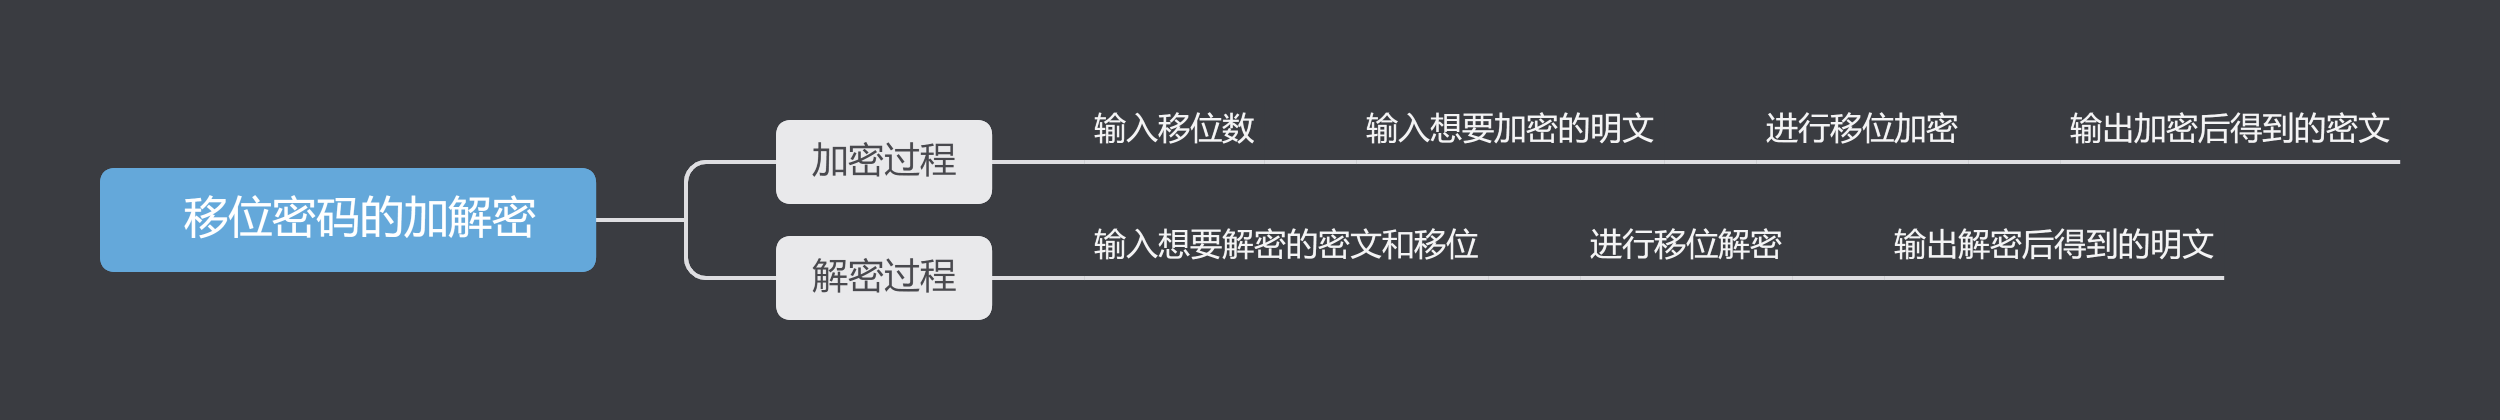
\includegraphics[width=16cm]{figure/figure1.png}
	\caption{移位密码的加解密流程}
	\label{fig:移位密码的加解密流程}
\end{figure}

\subsection{移位密码程序代码}
\begin{lstlisting}[language=c++]
#include <iostream>
using namespace std;

class shift_crypt
{
	private:
	int offset;//移位
	char* ciphertext;//密文
	public:
	shift_crypt()
	{
		offset = 0;
	}
	shift_crypt(int offset)
	{
		this->offset = offset;
	}
	char* get_ciphertext()
	{
		return this->ciphertext;
	}
	void shift_encrypt(char* plaintext) //加密
	{
		offset = offset % 26;
		//cout << "offset: " << offset << endl;
		int len = strlen(plaintext);
		//cout << "len: " << len << endl;
		this->ciphertext = new char[len];
		for (int i = 0; i < len; i++)
		{
			//cout << "plaintext[i]: " << plaintext[i] << endl;
			if (plaintext[i] >= 'a' && plaintext[i] <= 'z' || plaintext[i] >= 'A' && plaintext[i] <= 'Z')
			{
				char temp = plaintext[i] + offset;
				//cout << "temp: " << temp << endl;
				if (temp > 'Z' && plaintext[i]<='Z' || temp > 'z')
				this->ciphertext[i] = temp - 26;
				else
				this->ciphertext[i] = temp;
			}
			else
			{
				this->ciphertext[i] = plaintext[i];
			}
			//cout << "ciphertext[i]: " << ciphertext[i] << endl;
		}
		this->ciphertext[len] = '\0';
	}
	char* shift_decrypt(char* ciphertext, int offset)//解密
	{
		int len = strlen(ciphertext);
		char* plaintext = new char[len];
		for (int i = 0; i < len; i++)
		{
			if (ciphertext[i] >= 'a' && ciphertext[i] <= 'z' || ciphertext[i] >= 'A' && ciphertext[i] <= 'Z')
			{
				char temp = ciphertext[i] - offset;
				if (temp < 'a' && ciphertext[i] >= 'a' || temp < 'A')
				plaintext[i] = temp + 26;
				else
				plaintext[i] = temp;
			}
			else
			plaintext[i] = ciphertext[i];
		}
		plaintext[len] = '\0';
		return plaintext;
	}
	void exhaust_decrypt(char* ciphertext)//穷举
	{
		int offset;
		char* plaintext;
		for (offset = 0; offset <= 25; offset++)
		{
			plaintext = shift_decrypt(ciphertext, offset);
			cout << "移位为:" << offset << " 时明文为:" << plaintext << endl;
		}
	}
};
int main()
{
	char* plaintext = new char[1024];
	char* ciphertext = new char[1024];
	int offset;
	cout << "请输入移位:";
	cin >> offset;
	cout << "请输入要加密的明文:";
	cin >> plaintext;
	
	shift_crypt pro = shift_crypt(offset);
	pro.shift_encrypt(plaintext);
	char* temp1 = pro.get_ciphertext();
	cout << "移位加密后的密文为:" << temp1 << endl << endl;
	cout << "请输入要解密的密文:";
	cin >> ciphertext;
	char* temp2 = pro.shift_decrypt(ciphertext, offset);
	cout << ciphertext << "对应的明文为:" << temp2 << endl << endl;
	
	cout << "穷举攻击的密文为:"<<temp1 << endl;
	pro.exhaust_decrypt(temp1);
	return 0;
}
\end{lstlisting}

\subsection{程序运行结果}
\begin{figure}[thbp!]
	\centering
	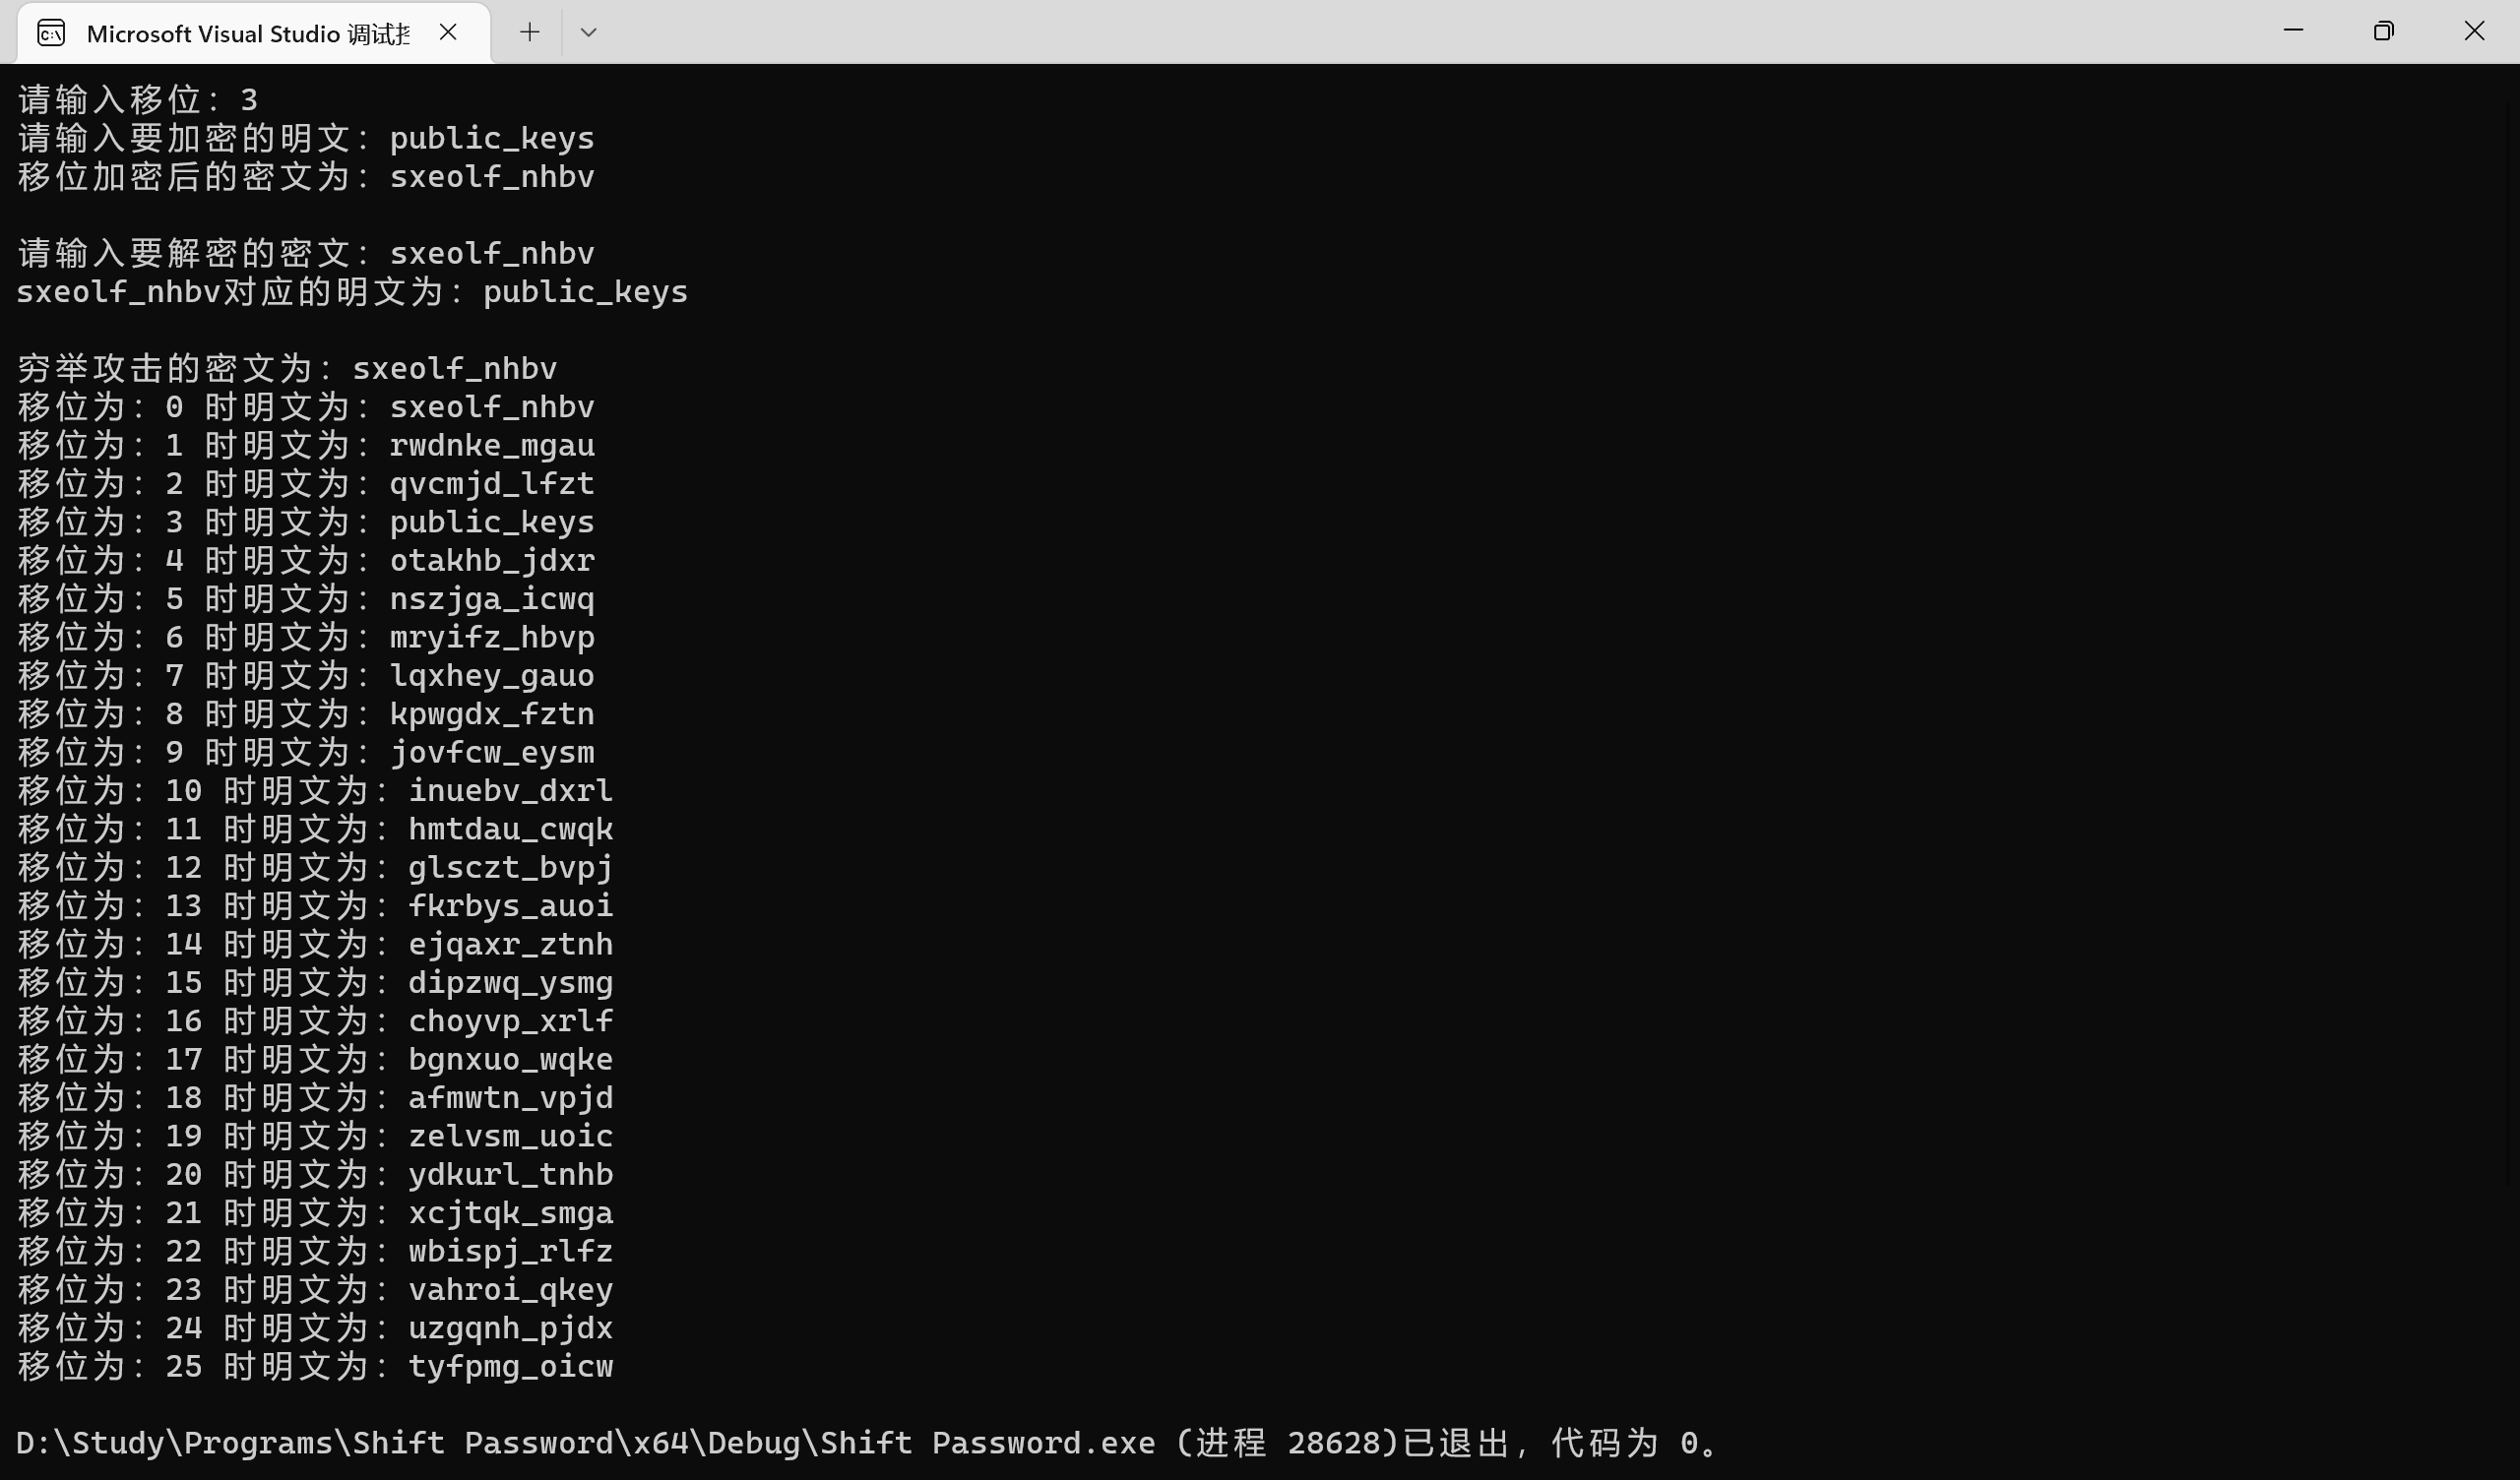
\includegraphics[width=16cm]{figure/002.png}
	\caption{移位密码加解密程序运行结果}
	\label{fig:移位密码加解密程序运行结果}
\end{figure}

%\begin{enumerate}
%	\item \textbf {预处理器:}处理源代码中以\#开始的预编译指令,例如展开所有宏定义、插入\#include指向的文件等,以获得经过预处理的源程序。
%	
%	\item \textbf {编译器:}将预处理器处理过的源程序文件翻译成为标准的汇编语言以供计算机阅读。
%	
%	\item \textbf {汇编器:}将汇编语言指令翻译成机器语言指令,并将汇编语言程序打包成可重定位目标程序。
%	
%	\item \textbf {链接器:}将可重定位的机器代码和相应的一些目标文件以及库文件连接在一起,形成真正能在机器上运行的目标机器代码。
%\end{enumerate}

%\begin{figure}[thbp!]
%	\centering
%	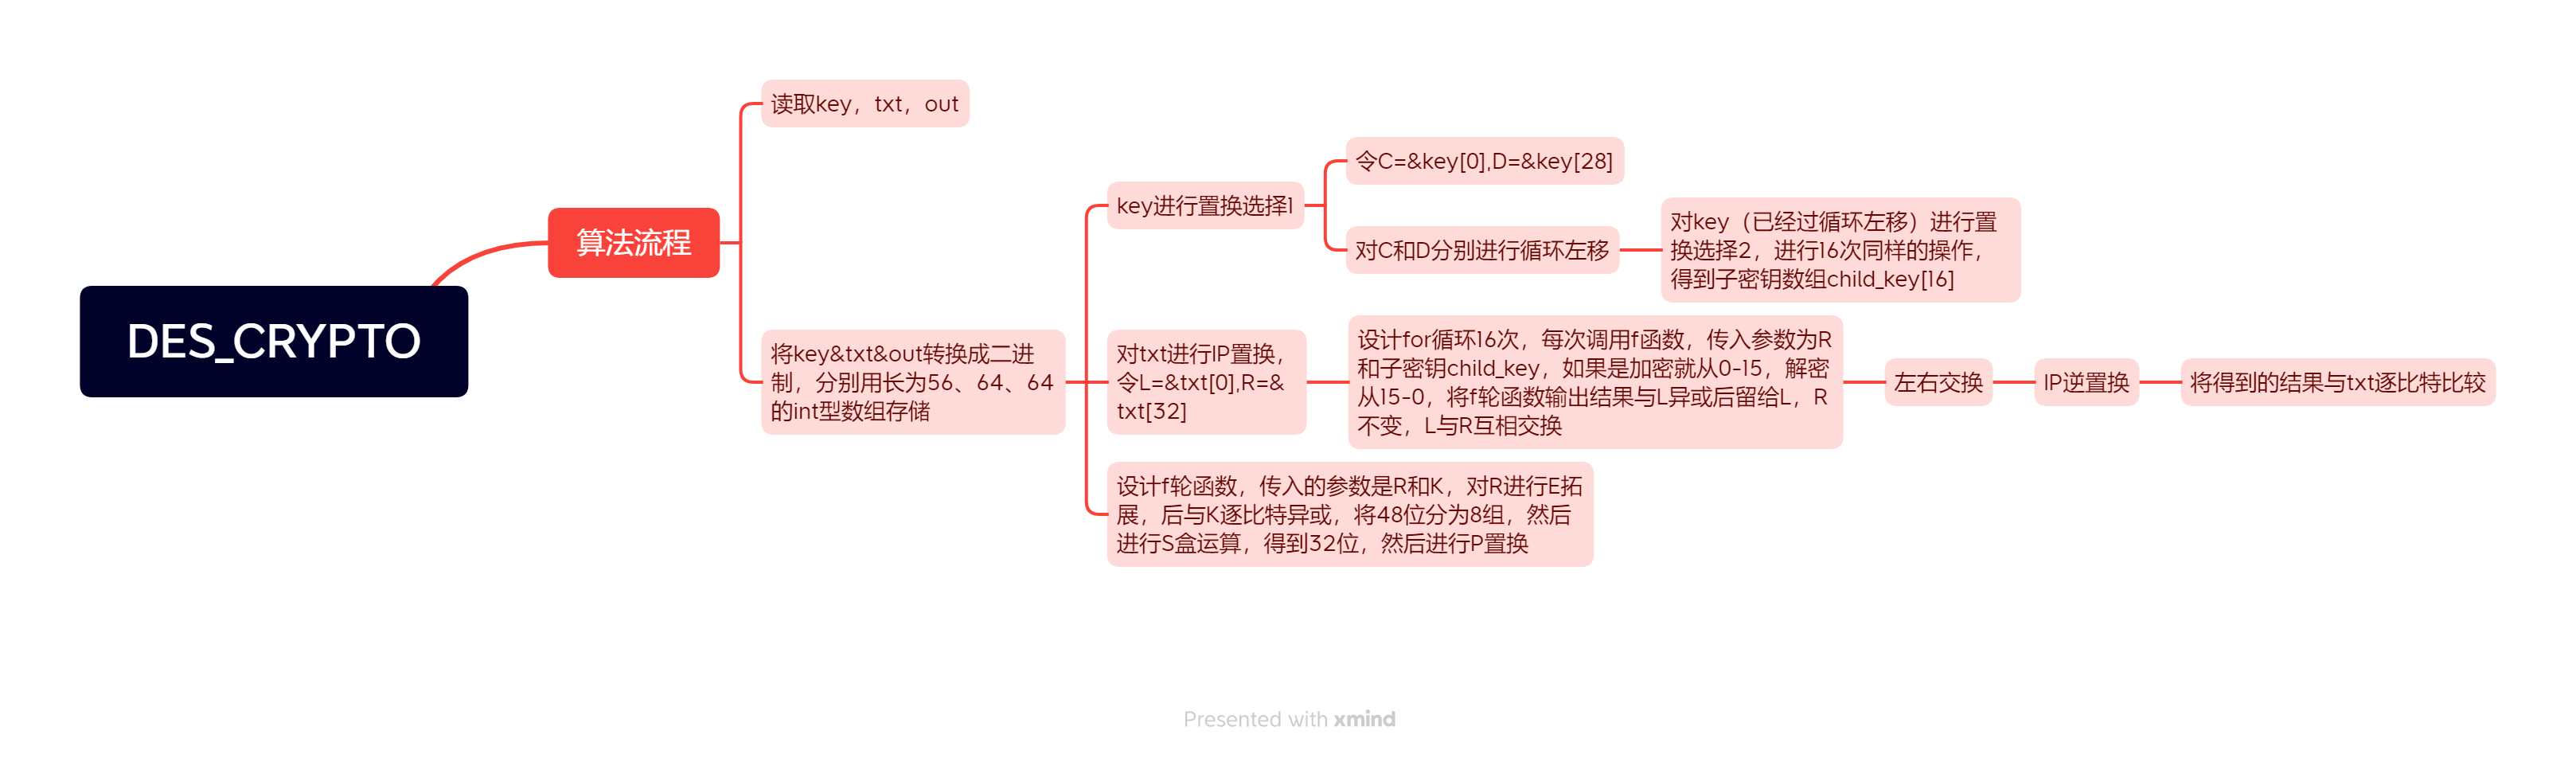
\includegraphics[height=6.8 CM]{figure/001}
%	\caption{语言处理过程图示}
%	\label{fig:语言处理过程图示}
%\end{figure}

























